%\documentclass[letterpaper]{article}
\documentclass[12pt]{article}

\usepackage[letterpaper, portrait, margin=1in]{geometry}

\usepackage{array}	% for \newcolumntype macro
\usepackage{caption}
\usepackage{graphicx}    % This package is used for Figures
\usepackage{rotating}           % This package is used for landscape mode.
\usepackage{epsfig}
\usepackage{comment}
\usepackage{url}
\usepackage{amsmath}
\usepackage{amssymb}
\usepackage{cite}
\usepackage{float}
\usepackage{hyperref}
\usepackage{subfig}
\usepackage{amsmath}
\usepackage{multirow}
\usepackage[T1]{fontenc}
\usepackage[all]{nowidow}
\usepackage[table]{xcolor}
\usepackage{siunitx}
\usepackage{listings}
\usepackage{notoccite}
\usepackage{grffile} % can use example.0.1.png
\usepackage{tabularx}		% Fill to margin on tables, control table width
\usepackage[normalem]{ulem}			% for strike through \sout{}
\usepackage{anyfontsize} % for the GIMP large letters
\usepackage{listings} % color the code
\usepackage{color} % to define colors
\usepackage{hhline} % to manually insert a vertical line with | or #
\usepackage{multicol} % Multiple columns
\usepackage{pgfplots} % Plotting in LaTeX
\usepackage{enumitem} % Globally change enumerate settings. Also allows for alpha/roman switch.
\setlist{nosep} % or \setlist{noitemsep} to leave space around whole list
\usetikzlibrary{arrows} % For triangular-headded arrows
\usetikzlibrary{patterns} % for patterns
\usepackage[thinlines]{easytable} % For simpler table commands

\newcommand{\degrees}{$^\circ$}
\newcolumntype{M}{>{\vspace*{1cm}\hfill}p{0.223\textwidth}<{\hfill\vspace*{1cm}}} % Middle aligned

\usepackage{fancyhdr} % To create headers
\pagestyle{fancy}
%\rhead{Dr. Kunz}
\newcommand{\docTitle}{Current and Circuits}
\chead{PHYS 2250 \docTitle}
\begin{document}
	\section*{Purpose}
	In this lab you will build a very simple circuit and use it to predict and measure the conductive properties of wires of different lengths and sizes.
	\section*{Introduction}
	Nichrome (NiCr) is a metal alloy of nickel and chromium with a very low electron mobility. The properties of Nichrome are shown in Table \ref{tab1}.
	
	In this lab, you will apply a voltage to Nichrome wires of different thicknesses and lengths. To get wires of different lengths, you will simply attach clip leads at different locations along the wires -- you will not cut the wires.
	\begin{table}[ht]
		\centering
		\begin{tabular}{|c|c|}
			\hline
			\textbf{Property} & \textbf{Value} \\
			\hline
			Electron density ($n$) & $9\times10^{28}\ \mathrm{m}^{-3}$\\
			\hline 
			Electron mobility ($u$) & $7\times10^{-5}\ \frac{\mathrm{m}/\mathrm{s}}{\mathrm{N}/\mathrm{C}}$\\
			\hline 
			Charge carrier & electron \\
			\hline
		\end{tabular}
		\caption{}
		\label{tab1}
	\end{table}

\begin{figure}
		\centering
		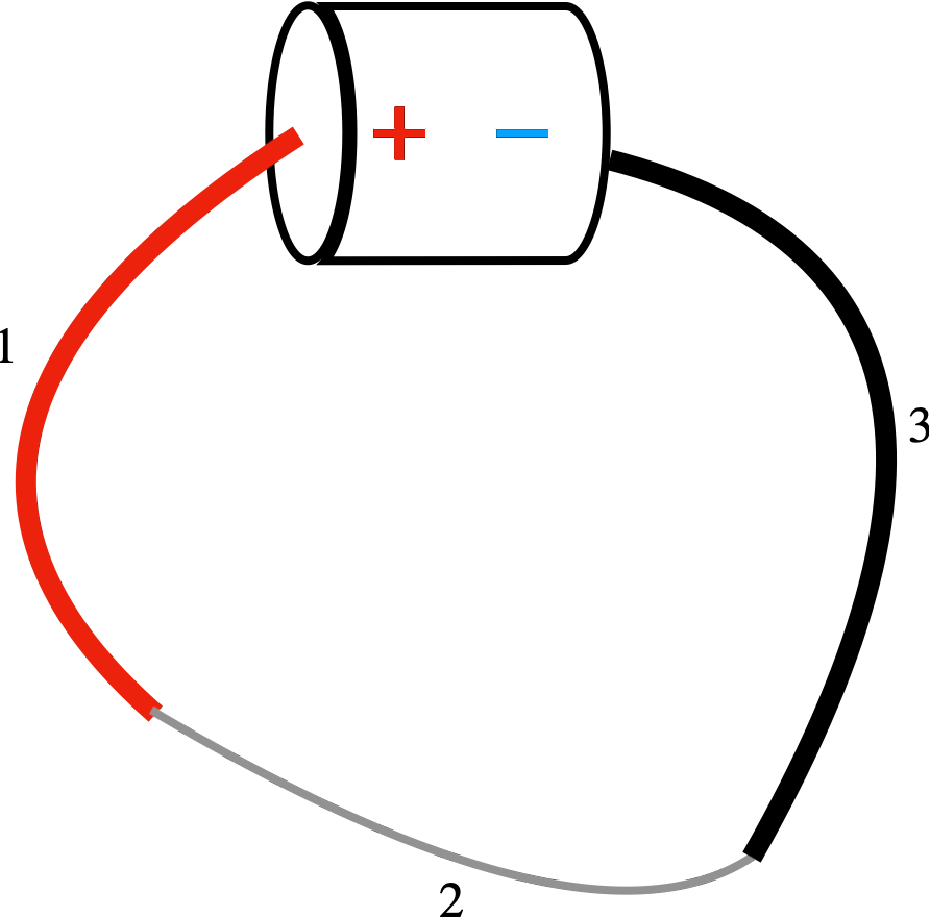
\includegraphics[width=.75\textwidth]{labfig}
		\caption{}
		\label{fig1}
\end{figure}

	\section*{Procedure}
		\subsection*{The Connecting Wires}
		The purpose of this lab is to investigate the affect that different lengths and thicknesses of nichrome wires has on the current flowing through the circuit. Normally, we can ignore the connecting wires in circuits, but the nichrome has similar conductive properties as the connecting wires. In the first part of the lab, we will measure the conductive properties of the connecting wires in order to isolate the affect of nichrome later on the lab.
		\begin{enumerate}
			\item Begin by connecting the two leads of the power supply through an ammeter, with nothing else connected. (Do not turn on the power supply; have your instructor approve the circuit).
			\item The loop equation for this circuit is
			\begin{equation*}
				\varepsilon-E_1L_1-E_2L_2-E_3L_3-E_4L_4=0
			\end{equation*}
			We can use the electron current relation $i=nAuE$ to rewrite the loop equation:
			\begin{equation*}
				\varepsilon-\frac{iL_1}{n_1A_1u_1}-\frac{iL_2}{n_2A_2u_2}-\frac{iL_3}{n_3A_3u_3}-\frac{iL_4}{n_4A_4u_4}=0
			\end{equation*}
			Or
			\begin{equation}
				\varepsilon - \left(\frac{L_1}{n_1A_1u_1}+\frac{L_2}{n_2A_2u_2}+\frac{L_3}{n_3A_3u_3}+\frac{L_4}{n_4A_4u_4}\right)i=0
				\label{eqn1}
			\end{equation}
			The term $\frac{L_1}{n_1A_1u_1}+\frac{L_2}{n_2A_2u_2}+\frac{L_3}{n_3A_3u_3}+\frac{L_4}{n_4A_4u_4}$ will appear in our loop equations later on. We don't need to know the individual values, we only need the sum. We can obtain a number for this term by connecting the circuit to a known voltage $\varepsilon$ and measuring the resulting current $i$.
			\item Turn on the power supply at a low voltage, around 0.5 V, and measure the current. The multimeter calculates the mean of many current measurements automatically. Use the mean and standard deviation for your measurement and uncertainty.
			\item Now you can use Equation \ref{eqn1} to solve for $\frac{L_1}{n_1A_1u_1}+\frac{L_2}{n_2A_2u_2}+\frac{L_3}{n_3A_3u_3}+\frac{L_4}{n_4A_4u_4}$. We will call this term $r_\mathrm{wires}$, since it looks very much like a resistor. Equation \ref{eqn1} then becomes $\varepsilon-ir_\mathrm{wires}=0$; solving for $r_\mathrm{wires}$ gives: $r_\mathrm{wires}=\frac{\varepsilon}{i}$. Record this result for later use. Your current measurement should have included an uncertainty, therefore your value for $r_\mathrm{wires}$ will also have an uncertainty. If the uncertainty of $I$ is $\Delta I$, then the uncertainty for $i$ is $\Delta i=\Delta I / 1.6\times10^{-19}$ C. The uncertainty for $r_\mathrm{wires}$ is then $\Delta r_\mathrm{wires}=\frac{\varepsilon}{i}\frac{\Delta i}{i}$.
		\end{enumerate}
	
		\subsubsection*{Important: Measuring Current}
		When the multimeter is on, a live-updating estimate of the current is shown on the screen. Towards the bottom of the screen, the meter automatically keeps track of some statistics for you. You will use these for your current measurement.
		\begin{enumerate}
			\item When you are ready to measure current, press the \texttt{DC I} button (this is important as it refreshes the statistics). 
			\item The multimeter continually measures the current and calculates the mean and standard deviation for you. Wait until there are at least 10 measurements, then record these values. The mean is your estimate for the value of the current, the standard deviation is your estimate for the uncertainty.
		\end{enumerate}
	
		\subsection*{Investigating the Nichrome Wire}
		Now that we have quantified the effect of the connecting wires, we can play with the Nichrome. 
		\begin{enumerate}
			\item At your lab station are two pieces of nichrome wire, one thick ($A=0.327\ \mathrm{mm}^2$) and one thin ($A=0.128\ \mathrm{mm}^2$). Select a length of nichrome wire and place it in your circuit (so that it is connected to the power supply and in series with the ammeter). The effective length of the wire is the distance between the two clips that connect it to the circuit (to vary the length of the wire, simply move the clips closer together).
			\item Write the loop rule equation for this circuit and use it to predict the current that will be driven by a voltage of 1 V. Your prediction should also include an uncertainty, due to the uncertainty in your length measurements and the uncertainty in your $r_\mathrm{wires}$ measurement. The uncertainty is given by:
			\begin{equation*}
				\Delta i = \frac{\varepsilon}{i}\frac{ \sqrt{\left(\frac{\Delta L}{nAu}\right)^2+\Delta r_\mathrm{wires}^2}  }{\frac{L}{nAu}+r_\mathrm{wires}}
			\end{equation*}
			This calculation is done for you in the provided spreadsheet.
			\item Turn on the power supply and measure the current. Record your value. Remember to record both mean and uncertainty.
			\item Repeat your prediction and measurement three more times, varying the length and thickness of the wire until you have filled out Table \ref{tab2}.
		\end{enumerate}
	
	\section*{Analysis}
	\begin{enumerate}
		\item Were your predictions consistent with your measurements? Why or why not? Be quantitative.
		\item How fast were the electrons moving, on average, through the long, thick wire? What was the electric field in the wire?
	\end{enumerate}
	
	\begin{table}
		\centering
		\begin{tabular}{|p{2cm}|p{1.5cm}|p{1.5cm}|p{1.5cm}|p{1.5cm}|}
			\hline
			\textbf{Wire}&\multicolumn{2}{p{2cm}|}{\bfseries Predicted Current}&\multicolumn{2}{p{2cm}|}{\bfseries Measured Current}\\
			\hline
			%& $i$ & $\Delta i$ & $i$ & $\Delta i$ \\
			& \textbf{Mean} & \textbf{Uncert.} & \textbf{Mean} & \textbf{Uncert.} \\
			\hline
			Long + Thick&-&-&-&-\\
			\hline
			Short + Thick&-&-&-&-\\
			\hline
			Long + Thin&-&-&-&-\\
			\hline
			Short + Thin&-&-&-&-\\
			\hline
		\end{tabular}
		\caption{}
		\label{tab2}
	\end{table}
\end{document}
